\documentclass{standalone}
\usepackage{graphicx}	
\usepackage{amssymb, amsmath, amsthm}
\usepackage{color}

\usepackage{tikz}
\usetikzlibrary{arrows.meta, math}

\definecolor{light}{RGB}{220, 188, 188}
\definecolor{mid}{RGB}{185, 124, 124}
\definecolor{dark}{RGB}{143, 39, 39}
\definecolor{highlight}{RGB}{180, 31, 180}
\definecolor{lightteal}{RGB}{107, 142, 142}
\definecolor{midteal}{RGB}{72, 117, 117}
\definecolor{darkteal}{RGB}{29, 79, 79}
\definecolor{gray10}{gray}{0.1}
\definecolor{gray20}{gray}{0.2}
\definecolor{gray30}{gray}{0.3}
\definecolor{gray40}{gray}{0.4}
\definecolor{gray60}{gray}{0.6}
\definecolor{gray70}{gray}{0.7}
\definecolor{gray80}{gray}{0.8}
\definecolor{gray90}{gray}{0.9}
\definecolor{gray95}{gray}{0.95}

\tikzmath{
  % Horizontal position of center of circumcircle
  function circumcirclex(\xa, \ya, \xb, \yb, \xc, \yc) {
    return 0.5 * (  (\yc - \ya) * (\yc - \yb) * (\yb - \ya)
                  + (\xc * \xc - \xb * \xb) * (\yb - \ya)
                  - (\xb * \xb - \xa * \xa) * (\yc - \yb) ) / 
           ( (\xc - \xb) * (\yb - \ya) - (\xb - \xa) * (\yc - \yb));
  };
  % Vertical position of center of circumcircle
  function circumcircley(\xv, \xa, \ya, \xb, \yb, \xc, \yc) {
    return - (\xb - \xa) / (\yb - \ya) * (\xv - 0.5 * (\xa + \xb)) + 0.5 * (\ya + \yb);
  };
  % Slope of perpendicular bisector between two points
  function mperbi(\xa, \ya, \xb, \yb) {
    \m = ( \yb - \ya ) / ( \xb - \xa );
    return - 1 / \m;
  };
}

\begin{document}

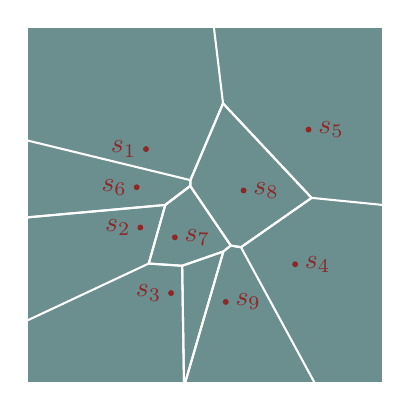
\begin{tikzpicture}[scale=1.5]
  \fill[lightteal] (-1.5, -1.5) rectangle (1.5, 1.5);
  \clip (-1.5, -1.5) rectangle (1.5, 1.5);
  
  \foreach \n/\x/\y in {4/0.765/-0.503, 5/0.878/0.637, 7/-0.254/-0.275, 8/0.328/0.122, 9/0.177/-0.822} {
    \fill[dark] (\x, \y) circle (0.025) node[right] { $s_{\n}$ };
  }
  
  \foreach \n/\x/\y in {1/-0.498/0.472, 2/-0.546/-0.192, 3/-0.286/-0.747, 6/-0.577/0.149} {
    \fill[dark] (\x, \y) circle (0.025) node[left] { $s_{\n}$ };
  }
  
  \draw[white, line width=0.75] (-0.475, -0.497)
    \foreach \x/\y in {-0.475/-0.497, -0.192/-0.516, 
                       0.157/-0.395, 0.220/-0.345, -0.124/0.160, 
                      -0.335/-0.001, -0.475/-0.497} {
      -- (\x, \y)
  };
  
  \draw[white, line width=0.75] (-0.251, -2.000)
    \foreach \x/\y in {-0.251/-2.000, -0.176/-1.538, -0.192/-0.516, -0.475/-0.497} {
      -- (\x, \y)
  };
  
  \draw[white, line width=0.75] (1.197, -2.000)
    \foreach \x/\y in {1.197/-2.000, 0.306/-0.359, 0.220/-0.345, 0.157/-0.395, -0.176/-1.538} {
      -- (\x, \y)
  };
  
  \draw[white, line width=0.75] (2.000, -0.050)
    \foreach \x/\y in {2.000/-0.050, 0.904/0.059, 0.306/-0.359} {
      -- (\x, \y)
  };
  
  \draw[white, line width=0.75] (0.017, 2.000)
    \foreach \x/\y in {0.017/2.000, 0.154/0.859, 0.904/0.059} {
      -- (\x, \y)
  };
  
  \draw[white, line width=0.75] (-2.000, 0.666)
    \foreach \x/\y in {-2.000/0.666, -0.122/0.209, 0.154/0.859} {
      -- (\x, \y)
  };
  
  \draw[white, line width=0.75] (-2.000, -0.151)
    \foreach \x/\y in {-2.000/-0.151, -0.335/-0.001, -0.124/0.160, -0.122/0.209} {
      -- (\x, \y)
  };
  
  \draw[white, line width=0.75] (-2.000, -0.151)
    \foreach \x/\y in {-2.000/-0.151, -0.335/-0.001, -0.124/0.160, -0.122/0.209} {
      -- (\x, \y)
  };
  
  \draw[white, line width=0.75] (-2.000, -1.212)
    \foreach \x/\y in {-2.000/-1.212, -0.475/-0.497, -0.335/-0.001} {
      -- (\x, \y)
  };
  
  \draw[white, line width=0.75] (-0.122, 0.209)
    \foreach \x/\y in {-0.122/0.209, -0.124/0.160, 0.220/-0.345, 0.306/-0.359, 0.904/0.059, 0.154/0.859, -0.122/0.209} {
      -- (\x, \y)
  };
  
  \draw[white, line width=0.75] (-0.176, -1.538)
    \foreach \x/\y in {-0.176/-1.538, 0.157/-0.395, -0.192/-0.516, -0.176/-1.538} {
      -- (\x, \y)
  };

\end{tikzpicture}

\end{document}  